\section{GUI Externes Design}

\begin{figure}[H]
  \begin{center}
    {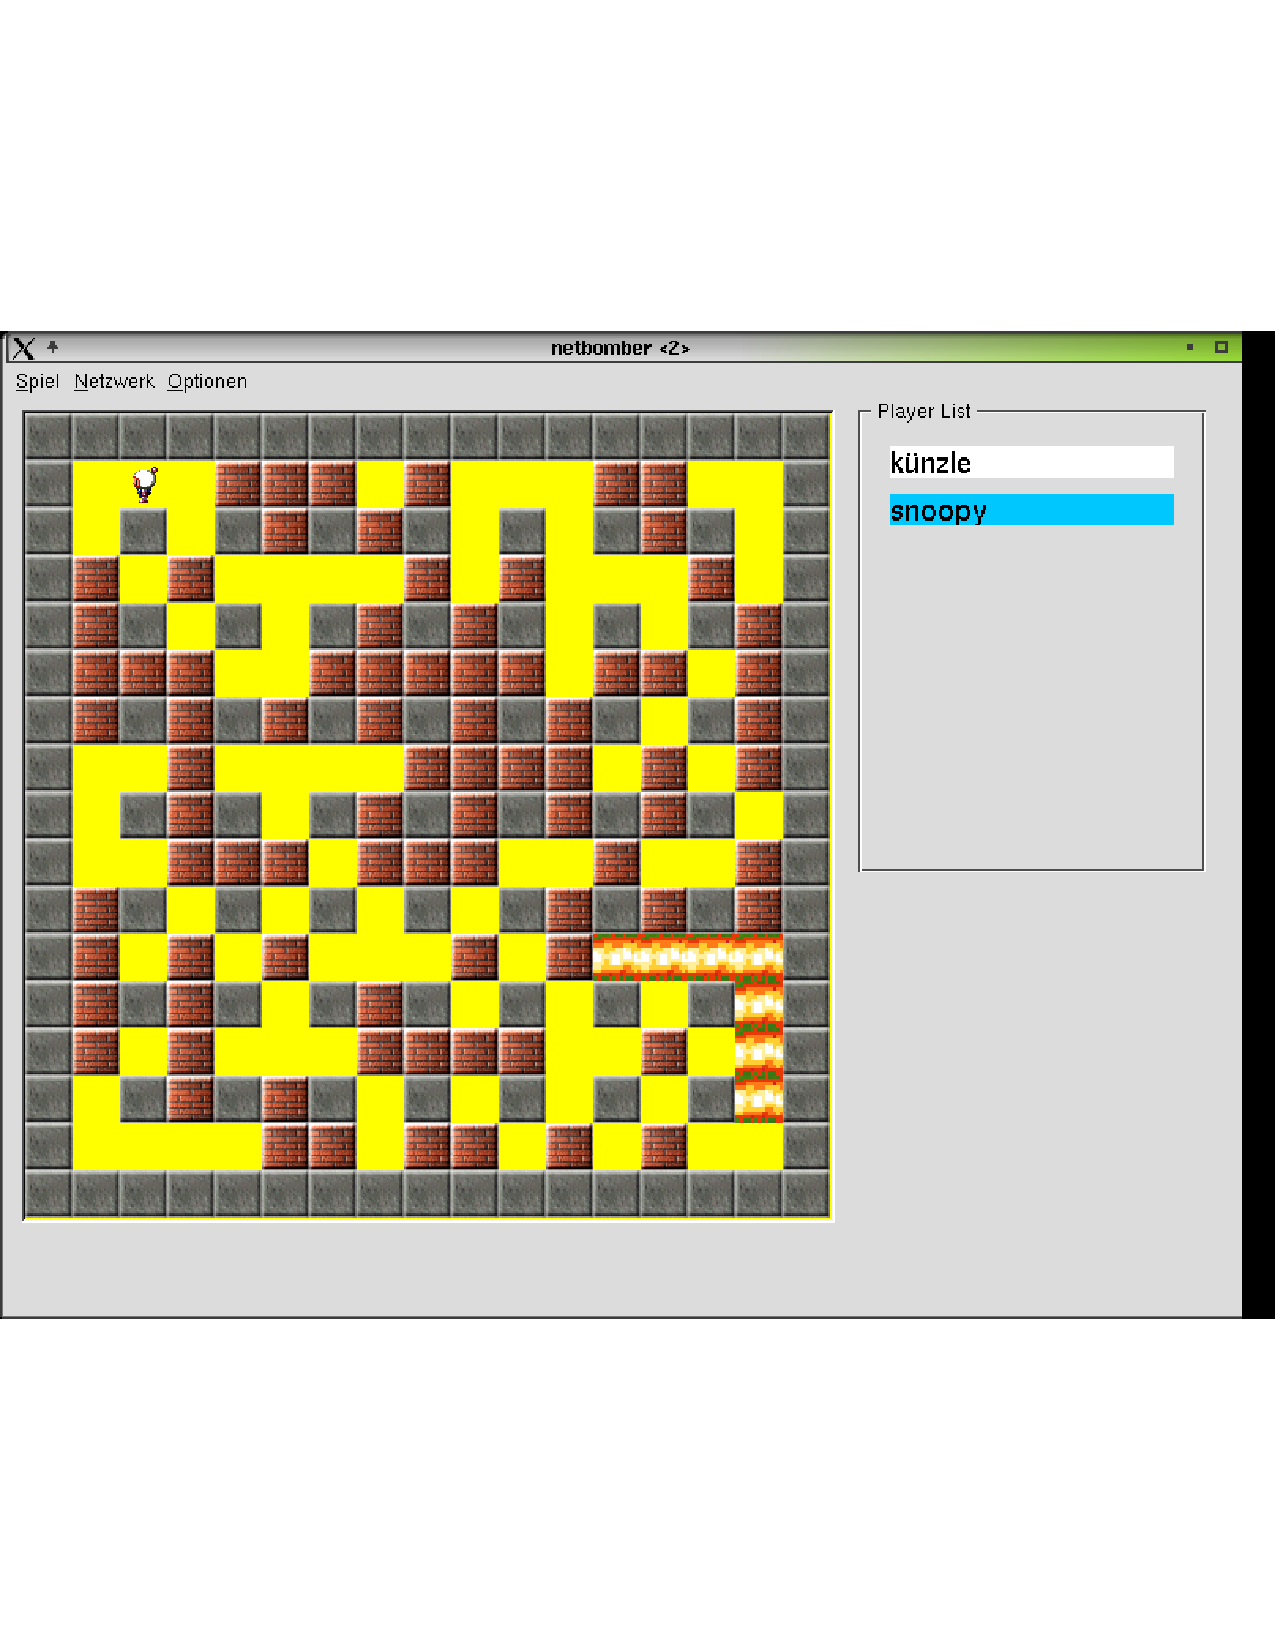
\includegraphics[height=12cm]{./images/spielfeld.pdf}}
  \end{center}
  \caption{Endversion des GUIs}
\end{figure}
Das Spielfeld (links) besteht aus diversen Spielelementen.
Diese werden dynamisch geladen, je nach dem was der Server
verlangt zum Darstellen. Rechts vom Spielfeld befindet sich
die Playerlist. Jeder Spielername wurde unterschiedlich
eingef"arbt, genau so wie die Farbe des entsprechenden Kopfes
der Spielfigur.

Die Farben der Spielfiguren:
\begin{table}[H]
	\begin{center}
		\begin{tabular}{|p{50mm}|p{30mm}|p{60mm}|}
		\hline Spielfigur 1 & Weiss & RGB (255, 255, 255) \\
		\hline Spielfigur 2 & Blau  & RGB (0, 200, 255) \\
		\hline Spielfigur 3 & Gr"un  & RGB (60, 255, 0) \\
		\hline Spielfigur 4 & Violet & RGB (255, 60, 255) \\
		\hline 
	\end{tabular}
	\end{center}
	\caption{Farben der Spielfiguren}
\end{table}


\begin{figure}[H]
  \begin{center}
    {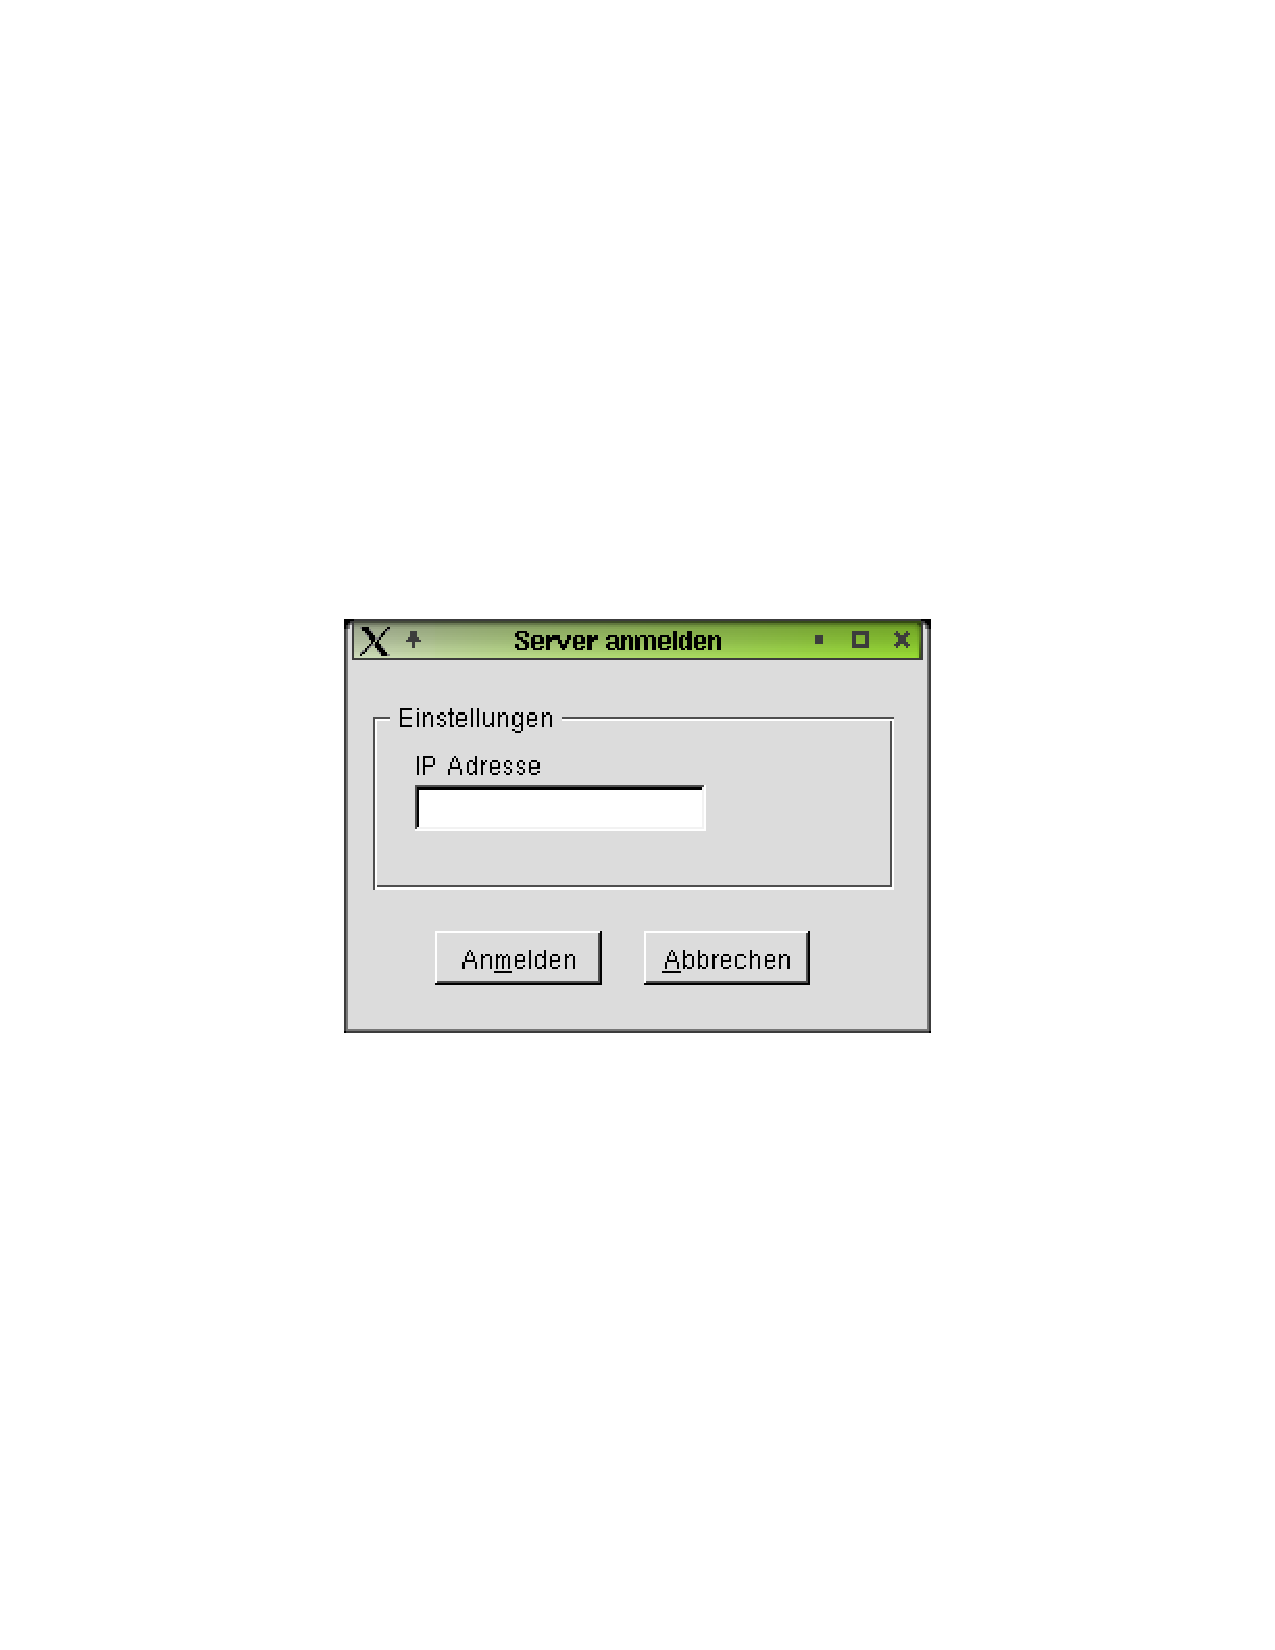
\includegraphics[height=6cm]{./images/joinserver.pdf}}
  \end{center}
  \caption{Snapshot des Dialoges Server anmelden}
\end{figure}

Dieser Dialog dient zum Anmelden an einen Server.

\begin{figure}[H]
  \begin{center}
    {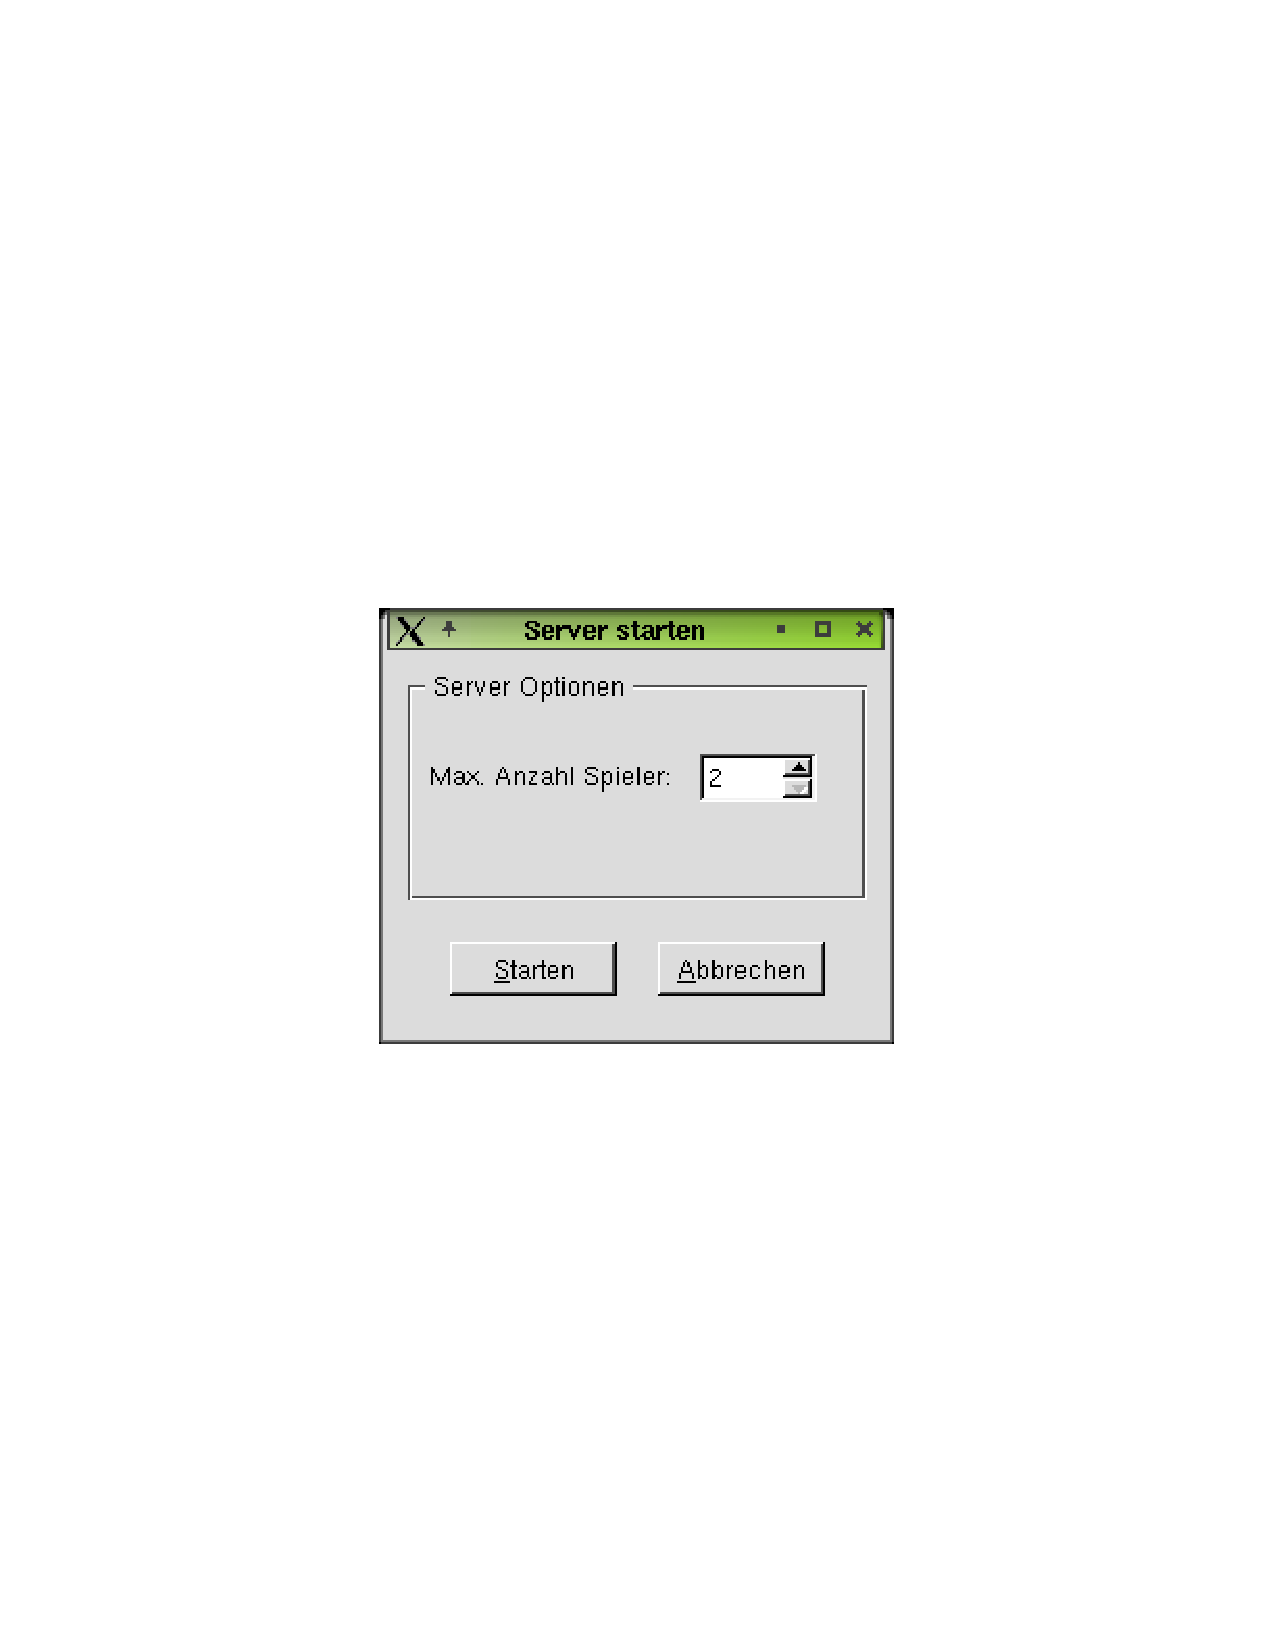
\includegraphics[height=6cm]{./images/startserver.pdf}}
  \end{center}
  \caption{Snapshot des Dialoges Server starten}
\end{figure}

Dieser Dialog dient zum Starten eines Servers.

\begin{figure}[H]
  \begin{center}
    {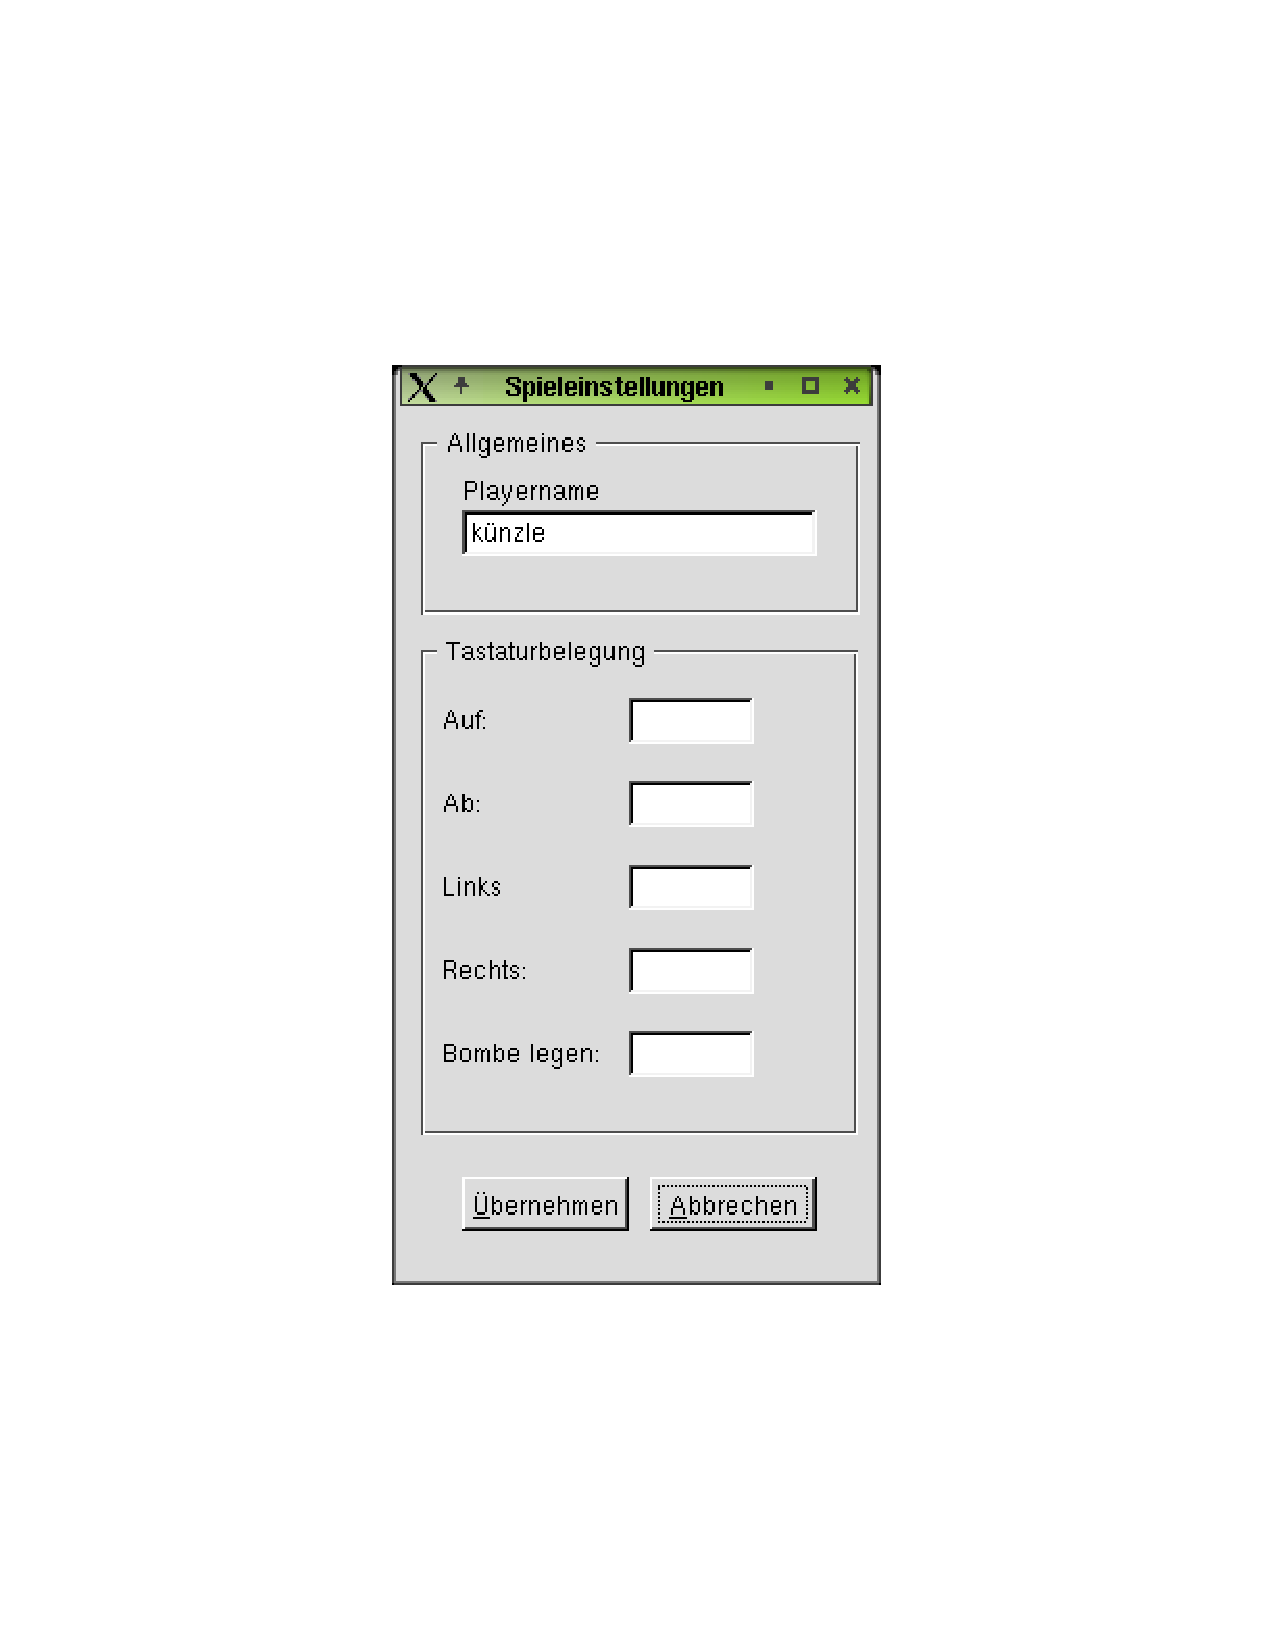
\includegraphics[height=10cm]{./images/settings.pdf}}
  \end{center}
  \caption{Snapshot des Dialoges Einstellungen}
\end{figure}

Dieser Dialog dient prim"ar zum Konfigurieren des Spielernamens.
Leider reichte uns die Zeit nicht mehr, die Tastaturbelegung
variierend zu machen. Vorgesehen war es jedoch in diesem Dialog.


\section{GUI Klassendiagramm}

Das gesamte Klassendiagramm befindet sich im Register Nr. 9.

\section{GUI Sequenzdiagramme}

\begin{figure}[H]
  \begin{center}
    {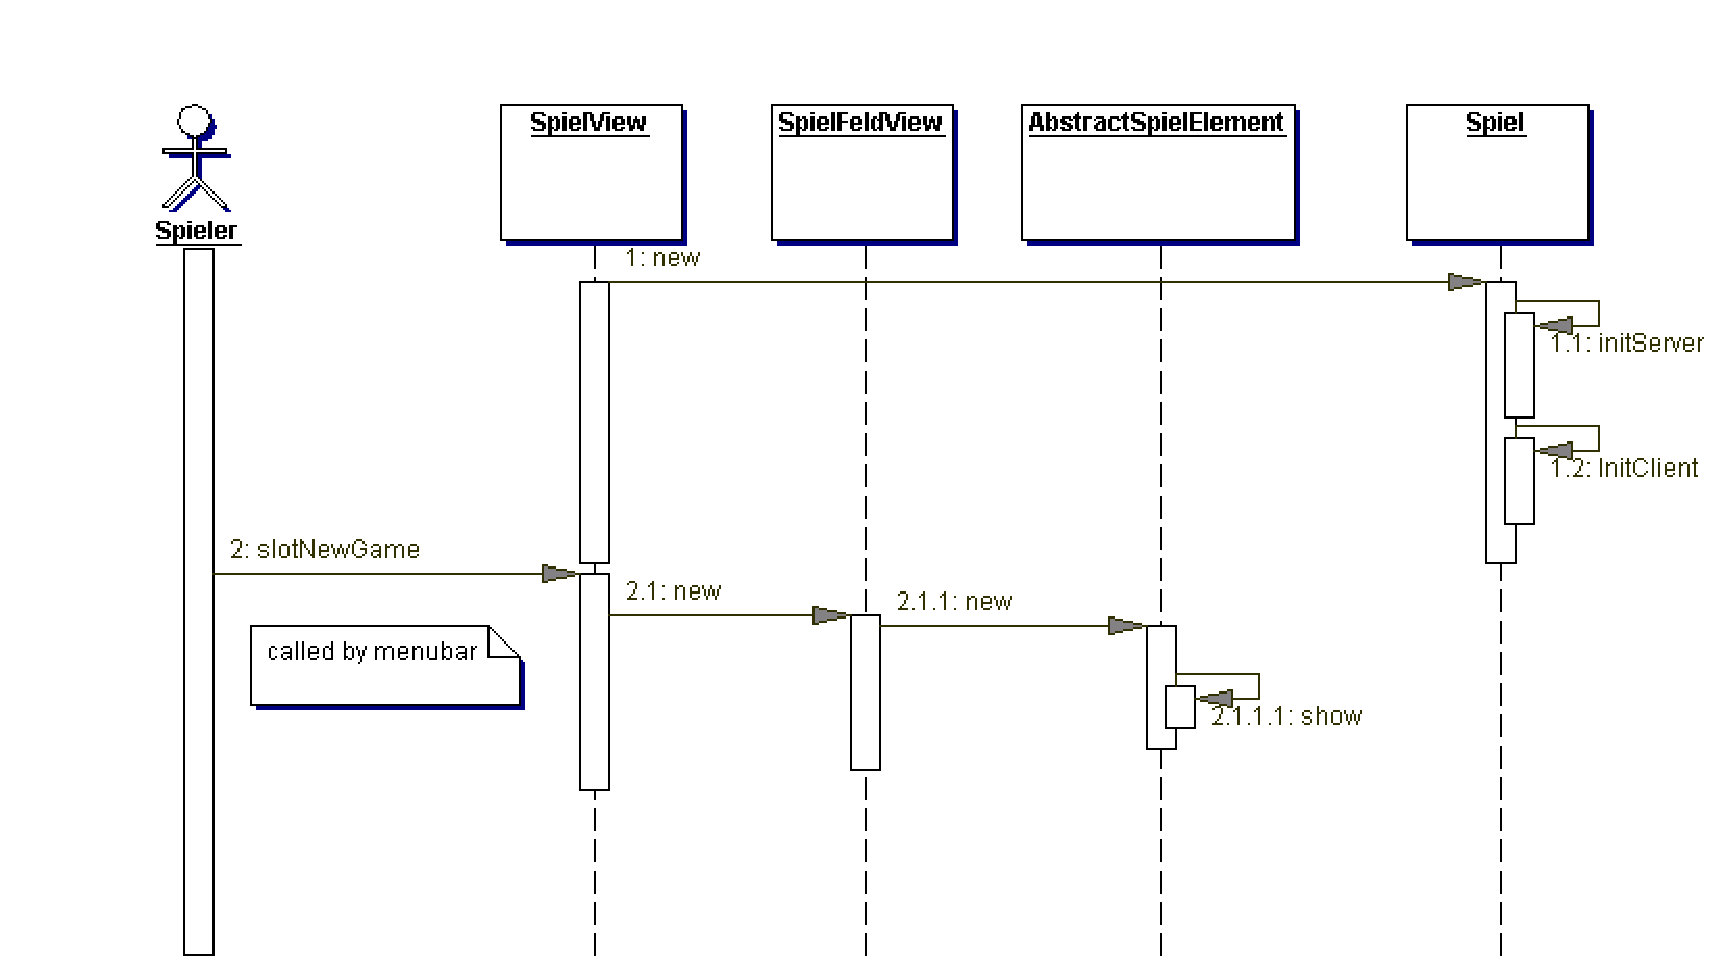
\includegraphics[height=6cm]{./images/neuesSpiel.pdf}}
  \end{center}
  \caption{Sequenzdiagramm f"ur neues Spiel}
\end{figure}



\begin{figure}[H]
  \begin{center}
    {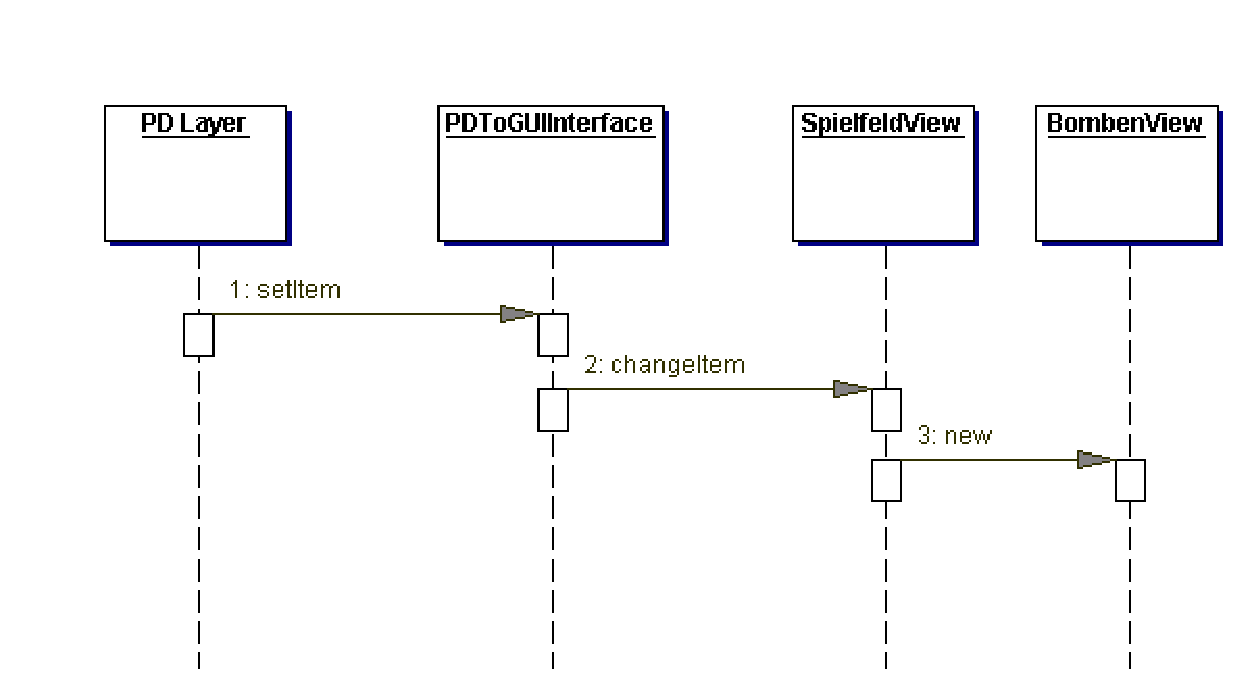
\includegraphics[height=6cm]{./images/bombeLegen.pdf}}
  \end{center}
  \caption{Sequenzdiagramm f"ur Bombe legen}
\end{figure}

Die PD wird hier als Blackbox betrachtet. Diese ruft "uber das
PDToGUIInterface setItem auf, wobei setItem als Parameter
den typ BOMBE und die Koordinaten x und y beinhaltet.
Die PDToGUIInterface Instanz teilt diese Anforderung der SpielfeldView
Instanz mit, welche dann mit dem Erzeugen einer neuen BombenView
Instanz reagiert.

\begin{figure}[H]
  \begin{center}
    {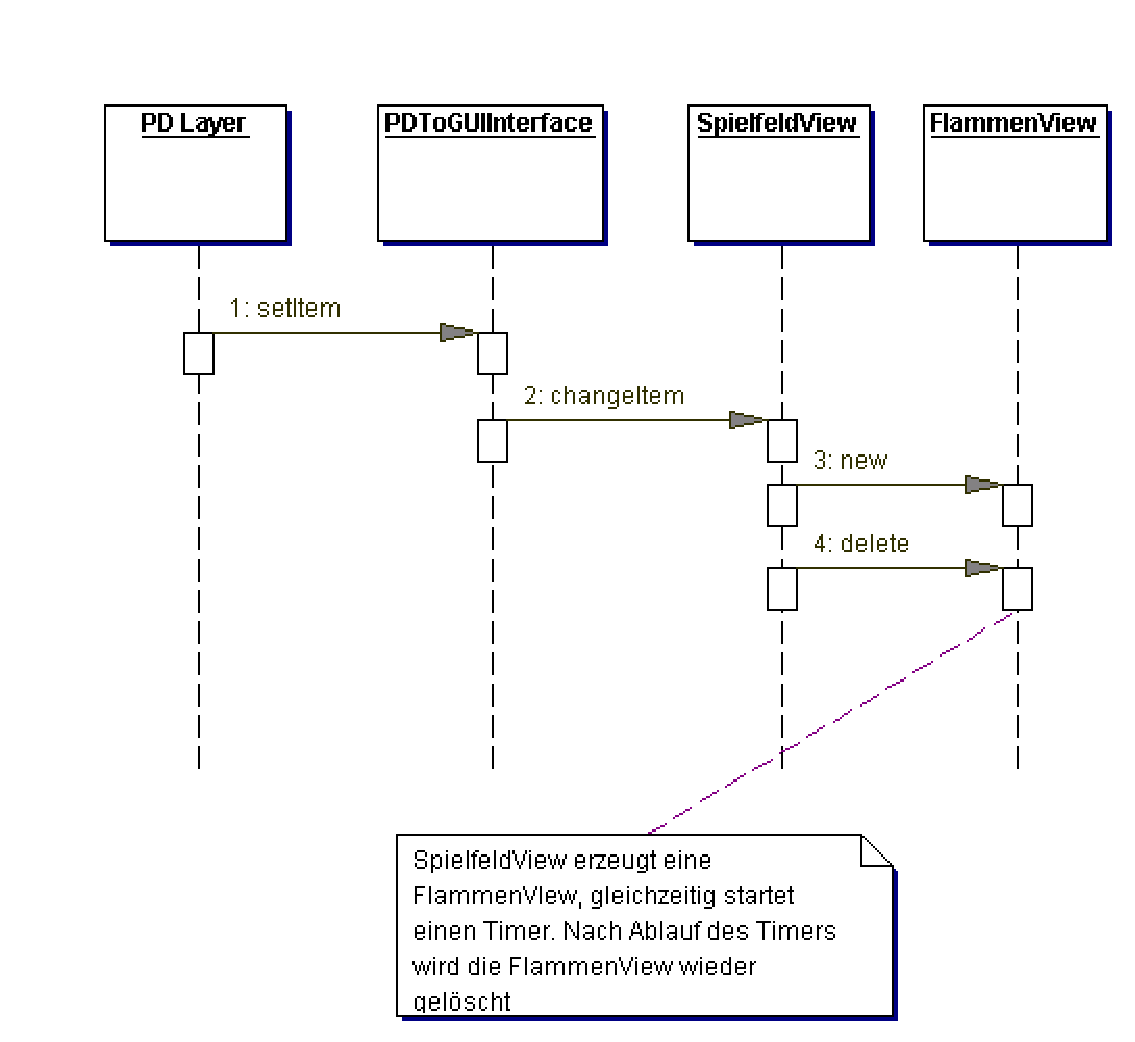
\includegraphics[height=6cm]{./images/neueflamme.pdf}}
  \end{center}
  \caption{Sequenzdiagramm f"ur eine Flamme anzeigen}
\end{figure}

Wieder vom PD Layer her kommt die Anforderung mit einem setItem.
Diesmal mit den Parametern FLAMME als typ und die Koordinaten x und y.
Die PDToGUIInterface Instanz leitet die Anforderung an die Instanz von SpielfeldView
weiter.
Die SpielfeldView Instanz erzeugt danach eine neue FlammenView Instanz. Gleichzeitig
startet einen Timer (QTimer), welcher nach Ablauf den Slot timerDone() aufruft.
In timerDone() wird die FlammenView wieder zerst"ort. Das bewirkt im Spiel selber
das kurze Erscheinen der Flamme, sozusagen explosionsartig.


\section{GUI Klassenbeschreibung}

\subsection{Klasse SpielView}

Die Klasse SpielView enth"alt einzig allein ein Menu. "Uber dieses kann der Spieler
einen Server starten, sich bei einem Server anmelden, Einstellungen vornehmen
und last but not least das Spiel starten bezw. beenden.
Um dies zu erm"oglichen, hat die Klasse SpielView Pointers auf die Klassen
JoinServerView, ServerView und SpielOptView. Diese werden bei den entsprechenden
Slots (Callbacks des Menus), mit show() aufgerufen.
Diese Klasse assoziiert ebenfalls mit der Klasse SpielFeldView, sozusagen
der Hauptklasse des GUIs (siehe unten). Im Konstruktur wird diese erzeugt, jedoch noch
nicht angezeigt. Dies erfolgt erst nachdem der Menupunkt Spiel starten ausgew"ahlt wurde.


\subsection{Klasse SpielFeldView}

Sie ist sozusagen die Kernklasse im GUI Design. Diese Klasse verwaltet alle
sich auf dem Spielfeld befindenen Elementen (Aggregation zu AbstractSpielElementView).
Um das zu erreichen, wird sie von der Klasse QCanvasView abgeleitet. QCanvasView
ist die Pr"asentationsklasse f"ur QCanvasItems, also f"ur einzelne Grafikelementen. Auch das
Keyboard-Eventhandling erfolgt in dieser Klasse. Falls Keyboard-Events auftreten,
werden diese abgefangen, und nur die f"ur das Spiel relevanten Steuersignale werden
der Klasse PDToGUIInterface weitergeleitet, wo sie dann von der PD verarbeitet werden.
Gleichzeitig erh"alt sie von der Klasse GUIToPDInterface Methodenaufrufe, welche das Ver"andern
des UI's zur Folge haben. Dies beinhaltet Items hinzuf"ugen und entfernen (Bombe und Flamme),
die Richtung der Spielfigur festlegen (um das entsprechende Sprite zu laden) und die Figur an
eine andere Koordinate bewegen. Um die Spielfigur eindeutig zu identifizieren, hat die Methode
moveXY() zus"atzlich den Paramter ID, dessen Wert die PD weiss.
Diese Klasse ist fast intelligenzlos. Sie nimmt nur Befehle von der Interfaceklasse entgegen,
oder leitet an diese Steuersignale weiter.

\subsection{Klasse SpielfigurView}

Diese Klasse repr"asentiert die Spielfigur. Sie wird im Konstruktor der Klasse SpielFeldView
erzeugt. Ihre Koordinaten erh"alt sie ebenfalls von der Klasse SpielFeldView.
Um grafisch ansprechende Animationen zu erm"oglichen, ist sie von der Klasse QCanvasSprite
abgeleitet. Diese Klasse erm"oglicht das dynamische Laden von Bildern (Frames), welche
durch entsprechende Methoden zu einer Animation zusammengesetzt werden k"onnen. In der Methode
advance(int step) erfolgt die eigentliche Animation in zwei Schritten: Wenn step 0 ist, hat
man die M"oglichkeit, die Items auf dem Spielfeld auf Kollision zu "uberpr"ufen (collision detection).
Im zweiten Schritt (step ist 1) werden die Items, in unserem Fall die Spielfigur, bewegt.
Diese Methode wird von Qt aufgerufen, vorausgesetzt das setAnimated(true) aiufgerufen wurde.

\subsection{Klasse AbstractSpielElementView}

Diese Klasse wurde von der Klasse QCanvasPolygonalItem abgeleitet. Sie erg"anzt diese
Klasse nur mit den Koordinaten. Gleichzeitig dient sie als Oberklasse f�r alle
auf dem Spielfeld befindenen Elementen, ausser der Spielfigur. Dies ist notwendig,
um die Aggregation zwischen SpielFeldView und AbstractSpielElement zu erreichen.

\subsection{Klasse MauerView}

Sie repr"asentiert auf dem Spielfeld eine unzerst"orbare Mauer. Das Attribut
rtti steht f"ur run time type information. Sie dient zur Identifikation.

\subsection{Klasse BombenView}

Sie repr"asentiert eine Bombe auf dem Spielfeld.

\subsection{Klasse FlammenView}

Sie repr"asentiert eine Flamme auf dem Spielfeld.

\subsection{Klasse ServerView}

Diese Klasse repr"asentiert einen Dialog, "uber welchen
einen Server gestartet werden kann. Als Option kann die
max. Anzahl Spieler festgelegt werden, nach dem Motto
""Server ist K"onig"".
Die Anmeldung erfolgt via den Klassen SpielView und GUIToPDInterface
zur PD mit dem Callback (Slot) bStartenPressed.

\subsection{Klasse JoinServerView}

Diese Klasse repr"asentiert einen Dialog, "uber welchen
sich ein Spieler an einen Server anmelden kann. Das einzige,
was der Spieler tun muss, ist eine g"ultige IP-Adresse
(bei welcher einen NetBomb Server gestartet wurde) eingeben.
Der Anmeldevorgang beginnt nach dem Dr"ucken des Anmelden-Buttons,
bezw. in der Methode bStartenPressed.

\subsection{Klasse SpielOptView}

Sie repr"asentiert einen Dialog, "uber welchen der Spieler
Einstellungen zur Spielersteuerung und seinen Playername
eingeben kann.

\subsection{Klasse GUIToPDInterface}

Sie ist die Kommunikations-Schnittstelle vom GUI zur PD.
Es werden die f"ur das Spiel relevanten Keyboard Events
zur PD weitergeleitet mit keyPressed und keyReleased.
Die PD erh"alt "uber die Schnittstelle die Aufforderung den
Server zu starten mit startServer(). Um sich an einen Server
anzumelden wird dir PD mit joinServer und den Parametern Spielername
bezw. IP  dies entsprechend mitgeteilt.
Um das Spiel schlussendlich zu starten, wird der PD mit startGame()
migeteilt.
Wir w"ahlten das Singleton Pattern der GoF, damit es einerseits nur
einmal instanziert ist, andererseits von jedem beliebigen Ort
zu Verf"ugung steht.

\subsection{Klasse PDToGUIInterface}

"Uber diese Klasse nimmt das GUI die W"unsche der PD entgegen. Alle
Aufrufe gehen danach weiter an die Klasse SpielFeldView.
Auch hier das Singleton Pattern der GoF aus den gleichen Gr"unden wie
bereits erw"ahnt wurde.

